\documentclass{scrreprt}
\usepackage[english]{babel}
% deutsche Umlaute
\usepackage[utf8]{inputenc}
\usepackage[T1]{fontenc}
\usepackage{lmodern}

% für das H placement Kommando bei figures:
\usepackage{float}

\usepackage{graphicx}
\usepackage{varioref}
\usepackage[
bookmarks=true,	% Lesezeichen erzeugen
bookmarksopen=false,	% Lesezeichen ausgeklappt
bookmarksnumbered=true,	% Anzeige der Kapitelzahlen am Anfang der Namen der Lesezeichen
pdfstartpage=1,	% Seite, welche automatisch geöffnet werden soll
%baseurl=http://www.server.de/dateiname.pdf, 
%  URL des PDF-Dokuments (oder Hintergrundinformationen)
pdftitle={STAV Report},
% Titel des PDF-Dokuments
pdfauthor={Johannes Schneider, Tim Henning},	% Autor(Innen) des PDF-Dokuments
%pdfsubject={},	% Inhaltsbeschreibung des
%pdfkeywords={},
% Stichwortangabe zum PDF-Dokument
breaklinks=true,	% ermöglicht einen Umbruch von URLs
colorlinks=true,	% Einfärbung von Links
linkcolor=black,	% Linkfarbe: schwarz (z.B. im Inhaltsverzeichnis)
anchorcolor=blue,	% Ankerfarbe: schwarz
citecolor=black, % Literaturlinks: schwarz
filecolor=black,	% Links zu lokalen Dateien: schwarz
menucolor=black, % Acrobat Menü Einträge: schwarz
pagecolor=blue, % Links zu anderen Seiten im Text: schwarz
urlcolor=black,	%  URL-Farbe: schwarz
%backref=true,
pagebackref=false,
pdfcenterwindow=true,
pdfnewwindow=true,
pdffitwindow=true,
pdfstartview=FitH,
pdfpagemode=UseOutlines
]{hyperref}
\usepackage{cleveref}

\usepackage{listings}
\lstdefinestyle{mystyle}{
	breakatwhitespace=false,         
	breaklines=true
}
\lstset{style=mystyle}
\lstset{
	language=C++,
	basicstyle=\ttfamily,
	keywordstyle=\color{blue}\ttfamily,
	stringstyle=\color{red}\ttfamily,
	commentstyle=\color{green}\ttfamily,
	morecomment=[l][\color{magenta}]{\#}
}
% commands to skip lines:
\lstset{numbers=left,numberblanklines=false,escapeinside=||}
\let\origthelstnumber\thelstnumber
\makeatletter
\newcommand*\Suppressnumber{%
	\lst@AddToHook{OnNewLine}{%
		\let\thelstnumber\relax%
		\advance\c@lstnumber-\@ne\relax%
	}%
}

\newcommand*\Reactivatenumber[1]{%
	\setcounter{lstnumber}{\numexpr#1-1\relax}
	\lst@AddToHook{OnNewLine}{%
		\let\thelstnumber\origthelstnumber%
		\refstepcounter{lstnumber}
	}%
}
\makeatother


\title{TAV - Report}
\subtitle{Project: Luminosus}
\author{Johannes Schneider and Tim Henning}

\begin{document}

\maketitle

\tableofcontents

\setcounter{chapter}{-1}
\chapter{Application Selection}

\section{Introduction}

Modern lighting desks used to control the stage technique in large theaters and concert halls are complex embedded system, often running a proprietary software on a Linux or Windows system in combination with two or more multitouch screens and custom hardware like faders and encoders. They are connected to all the systems in an event location like house- and stage lights, projectors, hoists and sometimes even the sound equipment. For communication between the components the industry recently started to use standardized network protocols.

Extending the functionality of such a lighting desk can be a difficult and time consuming task. To make it easier to integrate and test new features, the idea was to create a separate modular software platform that is connected via network to the lighting console. As a solution for this "Luminosus" was developed.

It is designed for lighting consoles from the market leader Electronic Theatre Controls (ETC) and uses the Open Sound Control (OSC)\footnote{see \textit{The Open Sound Control 1.0 Specification} by Matt Wright} protocol to control them. The user interface consists of modular function blocks that can be freely moved and connected. An example can be seen in \vref{fig:luminosus_example}.

\begin{figure}[h]
	\centering
	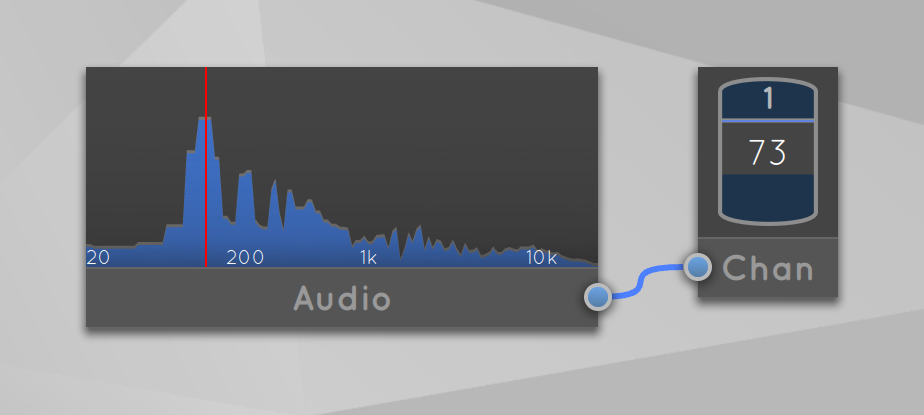
\includegraphics[width=0.75\textwidth]{img/luminosus_example}
	\caption[Luminosus Example]{Luminosus Example: Controlling the brightness of channel 73 by the current audio level}
	\label{fig:luminosus_example}
\end{figure}

The main project development was done by Tim Henning while writing his bachelor thesis. He is the only developer of the project until now. For this V\&V project Johannes Schneider joined the project as a developer and tester.

The programming language used is C++ 11 with syntax additions by Qt. The user interface part uses the declarative language QML\footnote{ sometimes referred to as 'Qt Modeling Language', see \url{http://doc.qt.io/qt-5/qtqml-index.html}} that includes function definitions in JavaScript.

The application is intended to be used by end users. It runs as a desktop application on Windows and MacOS and as an app on Android and iOS.

The existing code base consists of approximately 40k LOC (C++ source and header files + QML files). The code can be found on GitHub\footnote{\url{https://github.com/ETCLabs/LuminosusEosEdition}}.

Available artifacts are the source code, documentation, changelog\footnote{\url{https://github.com/ETCLabs/LuminosusEosEdition/blob/master/doc/Changelog.txt}}, issue tracker\footnote{\url{https://github.com/ETCLabs/LuminosusEosEdition/issues}}, manual\footnote{\url{https://github.com/ETCLabs/LuminosusEosEdition/blob/master/doc/Manual_en.pdf}} and in addition the Bachelor thesis \textit{Entwicklung einer modularen Benutzeroberfl\"ache als zus\"atzliche Bedieneinheit einer Lichtkonsole} including a requirement analysis and a discussion of the architectural decisions.

No specific development paradigm was used.

The current V\&V status is that only manual tests are performed (adding all available function blocks as a kind of \textit{smoke test} is available in the GUI) and static code analysis using Clang is provided by the IDE. Verification was not done yet.

\section{Learning from failures}

The following section is about learning from failures, which occurred over the course of developing the software.

\subsection{Issue \href{https://github.com/ETCLabs/LuminosusEosEdition/issues/2}{\#2} Connection to Eos stopped working:}

Since the software is basically an extension for an existing hardware device, the so-called lighting console, the most important component is the network connection to the said hardware. Should this component fail to execute its duties the entire software would become useless.
That said, this exact scenario appeared for a user during his show. The connection to his lighting console was interrupted for yet unknown reasons. Furthermore, the user was not able to pick up the lost connection even after restarting his entire setup, including multiple hardware components.

Although the fault is still undetected, it can be categorized as complexity related. This is, because the interaction of different devices in various environments is very hard to predict and even harder to test upfront. Reasons for this failure range from outdated driver software for the said hardware components over defective hardware up until a fault within the networking component of Luminosus.

\subsection{Issue \href{https://github.com/ETCLabs/LuminosusEosEdition/issues/3}{\#3} Faders not updated:}

The Eos lighting console offers a set of faders to control the light intensity on different devices. But since this set is very limited in the amount of supported devices, Eos additionally includes virtual pages of faders. Thus, the effective amount of hardware one can manage using the Eos lighting console increases immensely.

Luminosus also offers the feature of switching pages of faders. 

\begin{figure}[H]
	\centering
	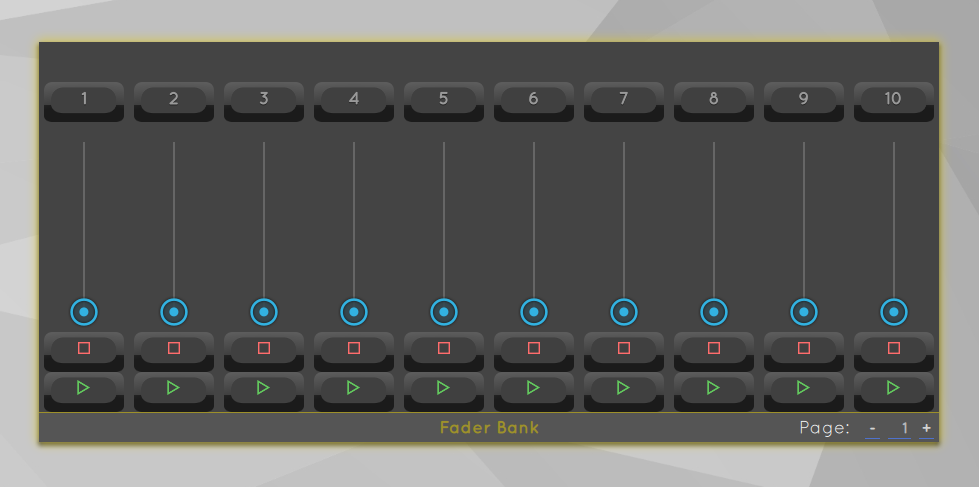
\includegraphics[width=0.75\textwidth]{img/luminosus_faders}
	\caption[Luminosus Fader Bank]{Luminosus Fader Bank: Visualization of the Eos faders including virtual pages}
	\label{fig:luminosus_faders}
\end{figure}

However, when switching between these pages, the corresponding faders were not updated properly. To be exact, they were not updated at all.

This failure was caused by a single missing line, which sets all faders to their initial position before requesting their current state. Thus, the fault was preventable, since a simple unit test could have covered this functionality.


\subsection{Issue \href{https://github.com/ETCLabs/LuminosusEosEdition/issues/4}{\#4} Fullscreen on iOS not working:}

Luminosus is designed to be cross-platform compatible. Thus, when working on a desktop computer most users would like Luminosus to be presented in fullscreen mode. This wish was realized by implementing a button, which offers just this functionality.
However, when running Luminosus on iOS, the fullscreen button caused the UI scaling to increase. This rendered the software practically unusable.

The exact cause for this failure is not discovered yet. Still you could say this failure was preventable by having a unit test which compares the scale property before and after the operation. However, the fault could also be treated as intelligent related, since the button should have not been enabled for mobile devices in the first place. So even if the function would have been working as expected, the resulting behavior would be irritating as the only difference of the fullscreen mode on a mobile OS is the removal of the status bar, which does not help the user at all.

\subsection{Conclusion}
In general the introduction of unit tests would be a valuable addition to the existing code base. Furthermore, integration tests for typical user scenarios would help to prevent many kinds of faults. Last but not least we learned that to maintain so many different platforms the user feedback is an important part in the process of V\&V.


\section{Five Basic V\&V Questions}

\paragraph{When do V\&V start?  When are they complete?}

Validation started right in the beginning. The project was validated on a daily basis  due to a lot of contact to the supervisor. The specification was adjusted very frequently to ensure that the features that were developed were suitable for the projects goal.

Analysis began early, too, in the form of static code analysis provided by the IDE (Qt Creator) and Clang. The development of tests did not start until the beginning of this V\&V lecture.

The process of V\&V does not end until the end of the lifetime of the product. In this case as long as the software is maintained.

\paragraph{What particular techniques should be applied during development?}

Static code analysis is very good applicable for C++ due to strict type declarations. 

Continuous Integration should be applied to the project since it will be used on various platforms. Furthermore, automated unit testing will be applied during the semester.

Additionally, profiling the memory consumption can help finding memory leaks and performance benchmarks make sure that the specification is met in terms of latency and responsibility.

In the end a formal verification of standardized components such as the network protocol implementations should be applied.

\paragraph{How can we asses the readiness of the product?}

The readiness is assessed by using the defined features of the specification and their current implementation status. Before a release is considered ready it should be at least tested manually in a typical use case scenario.

Furthermore, open issues are a hint that the product is not yet ready.

In the end the validation of a product is easier when the developer is also a user, as in our case. The greater the distance of the developer to the users of the product, the harder it is to match the use cases with the implementation. 

\paragraph{How can we control the quality of successive releases?}

To ensure that successive releases do not introduce new faults a pre-release policy can be established to let a small group of beta users test the system before it is released to the public.

The successful run of automated tests, especially regression tests, in a Continuous Integration environment can be a good indicator too.

\paragraph{How can the development process itself be improved?}

Increasing emphasis on applying various V\&V techniques during further development will help to improve overall code quality. 

Furthermore the development process can be improved by introducing a second developer to the project. Thus, pair programming and code reviews can be established to help finding flaws. In addition maintaining the documentation will lead to a better process.


\chapter{Analysis}

\section{Human-based Static Analysis}

The following section of about the peer review we performed. We figured out advantages and weaknesses of this technique.

\subsection{Peer Review}
\label{subsec:peer_review}

We organized our peer review sessions by picking suitable code snippets for each other. These snippets were supposed to be readable, even for someone who is not as deeply involved in the project or even the programming language at all. We then presented the selected code to the other group, while also introducing the general project. Afterwards, we further increased our understanding by asking questions about unclear syntax or general questions about details within the code. Finally, we were able to discuss issues and tried to find suitable solutions.

The code snippet we prepared is shown below.

\bigskip
\begin{lstlisting}[language=C++,
					numbers=left,
					firstnumber=171,
					directivestyle={\color{black}}
					emph={int,char,double,float,unsigned},
					emphstyle={\color{blue}},
					title=src/eos\_specific/EosCue.cpp]
void EosCue::createCueBlock() {
  EosCueBlock* block = qobject_cast<EosCueBlock*>(m_controller->blockManager()->addNewBlock("Eos Cue"));
  if (!block) {
    qWarning() << "Could not create Cue Block.";
  }
  block->setCueNumber(m_cueNumber);
  block->focus();
}
\end{lstlisting}
\bigskip

As requested, the code contained a fault. This fault was to be detected by our partners for the sake of this peer review.
The fault was a missing \texttt{return}-statement after line 174. This caused the function to continue its execution even when the \texttt{block} is a \texttt{nullptr}. Consequentially, line 176 would try to dereference this invalid pointer thus causing most likely an uncaught exception leading to a termination of the software.

After only a short while, our partners were able to locate and also fix the mentioned defect.

In return, they had a code snippet prepared for us which included a defect as well. 

% TODO: include code

When we finished understanding the context and general idea of the presented code, we were able to find the defect. Furthermore, we also suggested a change in the documentation, since it was misleading.

All together, our peer review session was mainly used for communication purposes and understanding the projects of each other. Additionally, the peer review helped us to exchange thoughts about various faults not only within our group but also with members of our partners group.

Main advantage of this kind of peer review is the fact, that every code snippet can be discussed directly with its author. This enables a very deep discussion about certain implementation decisions and also improves the overall code understanding by far. After just a short while, we were even able to detect a misleading documentation for a certain implementation, although we never saw the code before. 

In general, peer reviews can help to improve the product by selecting difficult code and talking about it in a very objective way. Thus, we do not need to play the blaming game and can just focus on finding and avoiding faults for future implementations. Additionally, it is very important to do this kind of analysis on a regular basis, so that the reviewed code is still manageable in size and difficulty. 

\subsection{Tools}

When performing peer reviews in a more professional way than we did, companies often use tools to support their process. The following section will evaluate some of the tools we already used.

\subsubsection{GitHub}

A tool we are very comfortable using is GitHub\footnote{\url{https://www.github.com}}. GitHub does not only allow you to host git repositories, so all your code is in just one place, but also offers a great variety of reviewing tools, like commenting coding line by line (see \vref{fig:github_review_comment}). The concept of pull requests and its support is also a very strong feature in GitHub. It offers developers a very formal way of merging branches into each other. It supports a human based review process by naming one or more reviewers for the pull requests. These reviewers may then comment, ask questions or suggest improvements for the code at hand. Although this process is mostly covered by the features offered by GitHub, we would like to have a way of (autonomously) selecting code of interest as we did in our peer review. Right now, every reviewer has to read all the code submitted for merging, making it very time consuming.

\begin{figure}[h]
	\centering
	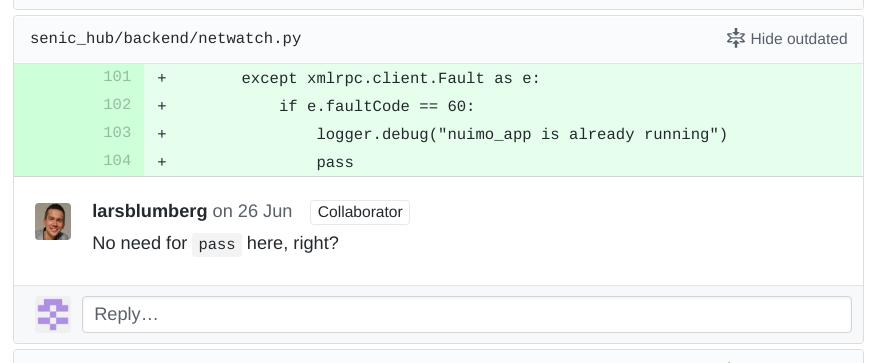
\includegraphics[width=0.9\textwidth]{img/github_review_comment}
	\caption[GitHub Review Comment]{A comment in the GitHub review tool}
	\label{fig:github_review_comment}
\end{figure}

While it is comfortable for the team members that these functions are integrated into the GitHub website and work in every browser, this also means that no code exploration features known from various IDEs are available. As a beginning it would be nice, for example, to be able to jump to a function declaration right from the review page of GitHub. This would help understanding the code a lot.

\subsubsection{SonarQube}

Besides GitHub, SonarQube\footnote{\url{https://www.sonarqube.org}} is another excellent web based tool for reviewing code. In contrast to GitHub, SonarQube is not used as a repository host. What makes SonarQube still great is its build-in fault detection and static analysis. Thus, a reviewer can find any flaws very fast and also see, who authored the corresponding code. We will cover more of the automated static analysis feature of SonarQube in section \ref{sec:humand-based-vs-automated-sa}.

What we missed when we used SonarQube was the possibility to see the entire commited code at once. SonarQube only offers to jump to fault it detected, but has no possibility to see the entire commit.

\section{Automated Static Analysis}

After we discovered and tested the human-based analysis of code, we also wanted to try automated analysis. Therefore, we chose tools, which are commonly used when analyzing C++ code. Our findings are documented in the following section.

\subsection{Clang Static Analyzer}

The first tool we tested was the Clang Static Analyzer\footnote{\url{https://clang-analyzer.llvm.org}}. We decided to test this tool not only because it has a great plugin for the IDE of our choice (Qt Creator\footnote{\url{https://www.qt.io/}}), but also because it is around for quite a while and therefore commonly known in the C++ community.

On the one hand, Clang helped to improve the code by finding a possible nullpointer dereference caused by a missing return statement (see \vref{subsec:peer_review}). 
On the other hand it reported hundreds of false alarms in its default configuration, i.e. increase of precision of floating point numbers thereby making it harder to detect the real faults (see \vref{fig:clang_fp_implicit_precision_increase}).

\paragraph{Inaccuracy}

The developers of Clang Static Analyzer clearly stated that the tool was made to reported as less false positives as possible. However, they are more concerned about not finding a fault, so they would tolerate a moderate amount of false alarms. This leaves us with the conclusion that the Clang Static Analyzer is mainly incorporating pessimistic inaccuracy, which results in false alarms. However, the tool can be configured to also include optimistic inaccuracy, if needed. This can be realized by adding filters so that some checks will become less strict. This behavior will result in some faults not being detected any longer.

\begin{figure}[H]
	\centering
	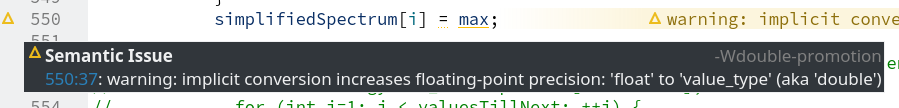
\includegraphics[width=0.9\textwidth]{img/clang_fp_implicit_precision_increase}
	\caption[Clang warns of increase in precision]{Clang warns of increase in precision of floating point number}
	\label{fig:clang_fp_implicit_precision_increase}
\end{figure}

Figure \ref{fig:clang_fp_implicit_precision_increase} is an example, of a very strict default configuration which leads to a false positive in our concrete project.

\subsection{Clang-Tidy} 

Next to the Clang Static Analyzer there is also the command line tool clang-tidy\footnote{\url{http://clang.llvm.org/extra/clang-tidy/}}. The tools are quite similar, the static analyzer focuses more on checks that require some sort of control flow analysis while clang-tidy includes linter-style checks and checks that are related to a certain coding style\footnote{see discussion here: \url{http://lists.llvm.org/pipermail/cfe-dev/2015-September/044966.html}}. Other than the static analyzer, clang-tidy is able to automatically fix most of the issues it found by modifying the source files directly, which is a very powerful feature to modernize legacy code bases.

In our case, clang-tidy was able to point out some hard to find readability issues such as a misleading use of static\_cast where dynamic\_cast would be more appropriate because it was a downcast from a base to a derived class. It also suggested good uses for the auto keyword, missing \texttt{override} keywords and showed function definitions where the variable names did not match those of the declaration. It even highlighted a case where a function call contained an inline comment with the name of the parameter (like '\texttt{foo(/*parameterName=*/ true)}') that did not match the real parameter name. After a quick configuration we were able to suppress most of the warnings related to a different coding style resulting in mostly true positives were shown.

\subsection{CppCheck} 

Although CppCheck\footnote{\url{http://cppcheck.sourceforge.net}} found faults which Clang missed, such as uninitialized member variables, we more disappointed for the most part. This is, because CppCheck claims to be designed to show as less false positives as possible, but still displayed a huge bunch of them for our project (see \vref{fig:cppcheck_fp_missing_ctor}).

\begin{figure}[h]
	\centering
	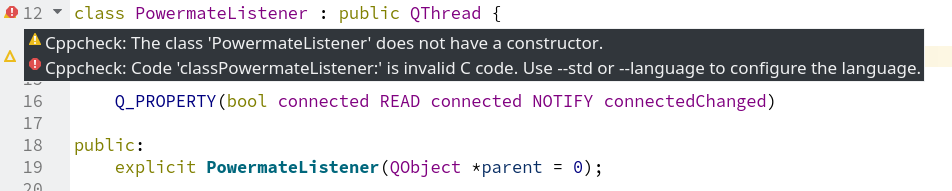
\includegraphics[width=0.9\textwidth]{img/cppcheck_fp_missing_ctor}
	\caption[Bugs in CppCheck]{Bugs in CppCheck result in false positives}
	\label{fig:cppcheck_fp_missing_ctor}
\end{figure}

This unwanted behavior is most likely caused by a bug in CppCheck itself, making it even more unsatisfying to use this tool in the first place.

\paragraph{Inaccuracy}

According to their website, the goal of CppCheck is to have zero false positives, resulting in a low pessimistic inaccuracy. They even recommend to use an additional tool that has a greater pessimistic inaccuracy, if required for the project. Unfortunately, in practice there are still some false positives, mainly related to bugs in CppCheck, as already mentioned before. The developers state that there are many faults that are not detected by CppCheck which leads to a high optimistic inaccuracy.

\subsection{Polyspace} 

Other than the previously shown tools, Polyspace\footnote{\url{https://www.mathworks.com/products/polyspace.html}} is a commercial product, which is made for industry standards of security critical environments. It claims to be capable of handling huge amounts of code and is also able to apply very in-depth analysis techniques, such as proofing the absence of some types of faults, like buffer overflows, division by zero and wrong array accesses\footnote{see \url{https://www.mathworks.com/products/polyspace-code-prover.html}}.

In the preparation of this report we tried to apply this tool to our project, but experienced some problems in using it (see \vref{fig:polyspace_analysis}). We were only able to validate one single source file, the only file with no dependencies other than the C++ standard library. To resolve the Qt includes, it would be necessary to monitor the build process of the project by Polyspace, which was not possible due to limited access to the system where Polyspace was installed on.

\begin{figure}[h]
	\centering
	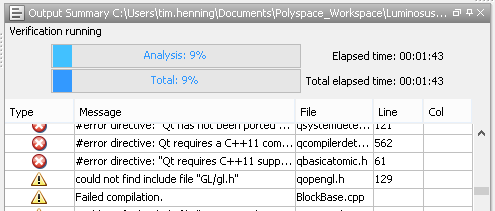
\includegraphics[width=0.7\textwidth]{img/polyspace_analysis}
	\caption[Polyspace Analysis]{Polyspace showing errors while analyzing C++ code with Qt dependencies}
	\label{fig:polyspace_analysis}
\end{figure}

\paragraph{Inaccuracy}

Polyspace is the only tool that we evaluated which claims to have zero optimistic inaccuracy for a specific set of faults. It realizes this by abstract interpretation of the code and automated formal validation methods.

\subsection{CppLint} 

A tool that is specialized in style guide checks is Googles cpplint.py\footnote{\url{https://github.com/google/styleguide/tree/gh-pages/cpplint}}. Even while this projects style guide differs from Googles, the tool can give some interesting hints. As an example, it was able to find missing includes that the other tools did not report. This is a valuable addition and shows again, that in the case of automated static analysis it is better to use a bunch of tools instead relying on a single one.

\section{Interaction between Human-Based and Automated SA}
\label{sec:humand-based-vs-automated-sa}

\begin{figure}[h]
	\centering
	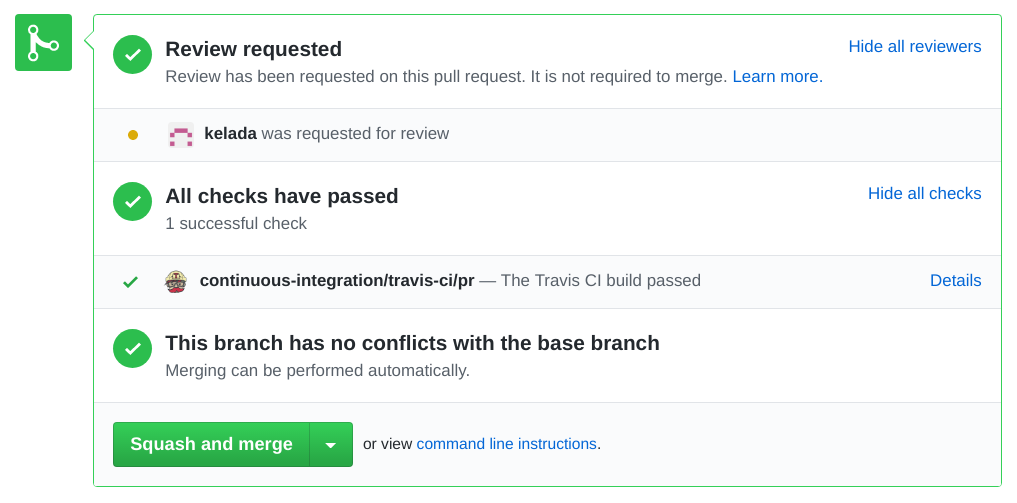
\includegraphics[width=0.9\textwidth]{img/github_pr_review}
	\caption[GitHub PR review]{Combination of ASA and human-based reviews in GitHub}
	\label{fig:github_pr_review}
\end{figure}

By using ASA a peer review can be prepared in order to point out potentially broken code parts. It can then be discussed if a detected fault is considered a false positive or not, and how to fix it. Additionally, some faults might be caused by a bad habit within the project team. These faults are very interesting to discover and can indicate certain lacks of the developing team, enabling more overall awareness once discussed thoroughly. They might even cause a change in the general consideration of good code in the team.  

When using tools like SonarQube, the faults get matched with their author. This enables each developer to learn from their mistakes in a more direct way. Additionally, it also displays which kind of faults are often produced in a project. These faults can then be targeted by further education and more awareness.

When thinking the other way around, the results of a human-based peer review can be used to improve the configuration of the automated static analysis tools. This can reduce the number of false positives which are caused by the coding guidelines of the individual project and thus are intended.
Depending on the use case, the relevance of faults is differently prioritized. In our specific case the implicit increase of precision of floating point numbers is not a problem at all. In contrast, in more space critical applications this could lead to unpredictable behavior.

In addition to the combination of ASA and human-based reviews, testing can also be integrated in this process. GitHub is a good example for this, as it shows the result of different software verification and validation methods at one glance, as seen in \vref{fig:github_pr_review}.

\chapter{Testing}

\section{Kick-off Tasks}

\subsection{Example Test Set}

As an example bug we chose issue \#17\footnote{\url{https://github.com/ETCLabs/LuminosusEosEdition/issues/17}}. It describes a problem where the application sometimes crashes when receiving cue objects. The following lines of code caused this:

\bigskip
\begin{lstlisting}[language=C++,
							numbers=left,
							firstnumber=78,
							directivestyle={\color{black}}
							emph={int,char,double,float,unsigned},
							emphstyle={\color{blue}},
							title=src/OSCNetworkManager.cpp]
void onIncomingEosMessage(const EosOSCMessage& msg) {|\Suppressnumber|
    [...]|\Reactivatenumber{92}|
    } else if (msg.path().size() <= 5) {
        // this message contains detailed information about a cue
        EosCueNumber cueNumber = EosCueNumber(msg.pathPart(2), msg.pathPart(3), msg.pathPart(4));|\Suppressnumber|
        [...]
\end{lstlisting}
\bigskip

The input data for a test case that leads to a failure would be a \texttt{msg} object with less than 5 path parts. The first error state would be that the program flow reaches line 94 with an \texttt{msg} object with less than 5 path parts. The fault is therefore in the if-condition in line 92 that evaluates to true because of the use of the '<=' operator instead of '=='. By trying to access the not existing 5th part of the path with \texttt{msg.pathPart(4)} in line 94 the program crashes with an index-out-of-bounds exception.

A test case that does not reach the fault is produced by using a \texttt{msg} object thats second path part is not 'cue'. This means the the message was not meant for this function, which is caught by an if-statement in the beginning that leads to an early exit prior to the fault.

The fault is reached but no error is produced if the \texttt{msg} object is correct and has 5 or more path parts.

It is not possible to create a test case that reaches the fault and produces an error without a failure. Each time line 94 is reached with an \texttt{msg} object with less than 5 path parts (the error state), the failure is visible by the index-out-of-bounds exception.

\subsection{Type of Existing Test Set}

There is no existing test set.

\subsection{Different Scopes of Test Case Execution}

A good example for a unit that can be tested at different scopes is the following function:

\texttt{QByteArray popPacketLengthFramedPacketFromStreamData(QByteArray\& tcpData) const}\footnote{\url{https://github.com/ETCLabs/LuminosusEosEdition/blob/master/src/OSCNetworkManager.cpp\#L306}}

Its purpose is to extract one valid OSC packet from a buffer of received network data. The packet should be removed from the buffer and returned as a QByteArray.

Testing the function in a small scope could be done by calling it with a previously prepared QByteArray buffer as the input data and comparing its output to the expected result and checking if the data was removed from the buffer.

At a medium scope the function \texttt{popPacketFromStreamData()} could be called after injecting the prepared data to the TCP socket object of the class. This method then checks which type of packet framing is used and eventually calls our function to test. It could then be checked the content of the packet is processed correctly in \texttt{processIncomingRawData()}.

In the end, the function should also be tested at a large scope by sending real data over the network to the application and observe if the data is processed correctly and the behavior is as expected. This is important as some characteristics of the system like buffer sizes in the network hardware are hard to predict or simulate and it ensures that the software works correctly in a real life scenario.

\section{Automated Unit Tests}

% TODO: this is just a collection of findings, needs to be rephrased

We are using the Google C++ Testing Framework\footnote{\url{https://github.com/google/googletest}} for automated tests.

\subsection{Google Test Setup}

Setting it up is rather simple: after installing the \textit{gtest} and \textit{gmock} libraries, it is possible to create a new executable that executes all available tests with only a few lines of code:

\bigskip
\begin{lstlisting}[title=tests/main.cpp]
#include <gtest/gtest.h>

int main(int argc, char[] argv) {
	::testing::InitGoogleTest(&argc, argv);
	return RUN_ALL_TESTS();
}
\end{lstlisting}
\bigskip

A very basic test could look like this:

\bigskip
\begin{lstlisting}[title=tests/Demo.cpp]
#include <gtest/gtest.h>

TEST(DemoTest, Add) {
	ASSERT_EQ(1+1, 2);
}
\end{lstlisting}
\bigskip

QtCreator has a basic Google Test integration. It can start all or only individual tests and displays the test results in the user interface.

\begin{figure}[h]
	\centering
	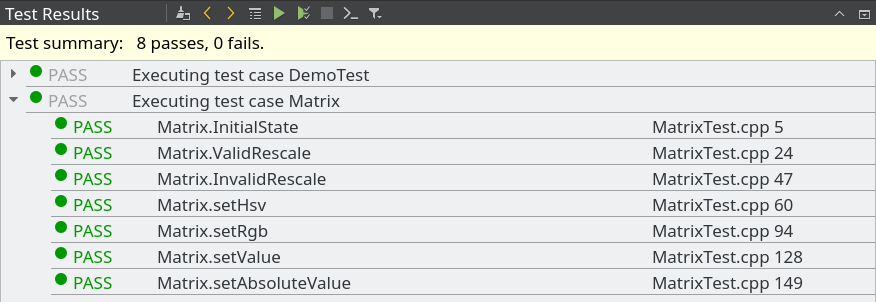
\includegraphics[width=1.0\textwidth]{img/qtcreator_test_results}
	\caption[QtCreator Test Results]{Test Results in QtCreator}
	\label{fig:qtcreator_test_results}
\end{figure}

\subsection{Code Coverage}

Unfortunately, it is not possible to calculate and display the code coverage of tests done with the Google Testing framework within QtCreator.

% TODO: find out how to calculate (and visualize?) coverage

\subsection{Bugs Found}

Even while writing the first few unit tests, we were able to identify some issues where the code was not behaving as expected.

In the first case an operation was never executed because of a wrong condition in an if-statement (rescaleTo() in Matrix.h).

Furthermore in the same class it was possible to set a variable to a higher or lower value than specified through its setter method. The expected behavior in this case would be that the variable is then limited to its upper or lower bound.



\end{document}
